\documentclass[10pt,a4paper]{report}
\author{Sara Terrón Ibáñez}
\usepackage[spanish]{babel}
\usepackage{amsmath}
\usepackage{amsfonts}
\usepackage{graphicx}
\begin{document}

\begin{titlepage}
\begin{center}
\begin{huge}
\vspace*{1cm}
\textsc{\hspace{1cm} \LaTeX \hspace{1cm} y \hspace{1cm} Git}\newline
\\[0.3cm]
\textsc{aplicado a la investigacion cientifica}\\
\vspace*{2.5cm}
\end{huge}
\begin{Huge}
\textbf{Ejercicio Final}\\
\end{Huge}
\vspace*{2.5cm}
\rule{90mm}{0.1mm}\\
\begin{Large}
\texttt{Autora:}\newline
\\[0.3cm]
\textsl{Sara Terron Ibanez}
\end{Large}
\end{center}
\end{titlepage}

\newpage
\tableofcontents

\chapter*{Tablas}
\addcontentsline{toc}{chapter}{Tablas}

Este es el horario que se seguira durante la realizacion del curso \footnote{Podra se modificado si se estima oportuno}.\ \\
\begin{center}
\begin{tabular}{|c|c|c|c|c|c|}
\hline 
\textbf{Horario} & \textbf{LUNES} & \textbf{MARTES} & \textbf{MIERCOLES} & \textbf{JUEVES} & \textbf{VIERNES} \\
\hline 
\textit{08:00h} & xxx & yyyy & zzzz & kkkk & yyyy \\ 
\hline 
\textit{09:00h} & yyyy & zzzz & xxxx & zzzz & kkkk \\ 
\hline 
\textit{10:00h} & xxx & yyyy & zzzz & kkkk & yyyy \\ 
\hline
\textit{11:00h} & \multicolumn{5}{|c|}{\textbf{DESCANSO}} \\ 
\hline
\textit{11:30h} & xxx & yyyy & zzzz & kkkk & yyyy \\ 
\hline 
\textit{12:30h} & yyyy & zzzz & xxxx & zzzz & kkkk \\ 
\hline 
\textit{130:30h} & xxx & yyyy & zzzz & kkkk & yyyy \\ 
\hline 
\end{tabular}
\end{center}


\chapter*{Listas}
\addcontentsline{toc}{chapter}{Listas}

\section{Lista enumerada \cite{Terron}}

Esto es una lista numerada:
\begin{enumerate}
\item Punto uno de la lista
\begin{enumerate}
\item Primer punto dentro de un punto
\item Segundo punto dentro de un punto
\end{enumerate}
\item Punto dos de la lista
\item Punto tres de la lista
\end{enumerate}
\ \\

\section{Lista marcada \cite{Ibanez}}

Esto es una lista marcada:
\begin{itemize}
\item Primer item lista
\begin{enumerate}
\item Punto numerado dentro de un punto
\item Otro punto numerado dentro de un punto
\end{enumerate}
\item Segundo item lista
\item Tercer item lista
\end{itemize}\ \\


\chapter*{Formulas}
\addcontentsline{toc}{chapter}{Formulas}

Algunas formulas matematicas con \LaTeX :\ \\

\begin{center}
$\Phi=\oint_{S}\overline{E}\cdot d\overline{S}=\frac{q_{enc}}{\varepsilon_{O}}$ \ (Ley\ de\ Gauss)\newline
\\[0.8cm]
$\oint_{S}\overline{E}\cdot d\overline{S}=0$\newline
\\[0.8cm]
$\oint_{C}\overline{E}\cdot\overline{dl}=-\frac{d}{dt}\oint_{S}\overline{B}\cdot\overline{dS}$\newline
\\[1cm]
\end{center}

Las siguientes funciones se muestran representadas en la figura \ref{grafica}.

\begin{center}
\begin{equation}
\mathbf{f=(x)=x}
\end{equation}
\end{center}
\begin{center}
\begin{equation}
\mathit{f(x)=\frac{1}{20}e^{x}}
\end{equation}
\end{center}
\begin{center}
\begin{equation}
\mathsf{f(x)=\sin x\:}
\end{equation}
\end{center}


\chapter*{Graficos}
\addcontentsline{toc}{chapter}{Graficos}

\begin{figure}[!h]
\begin{center}
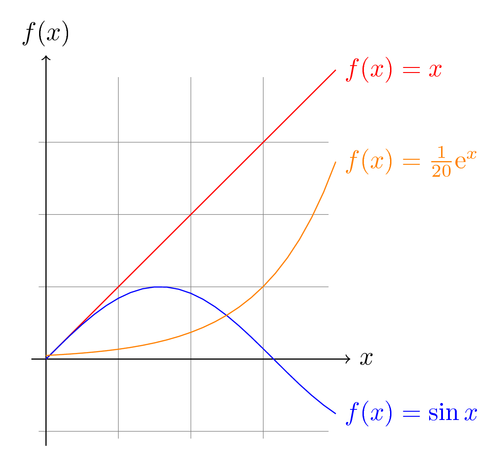
\includegraphics[scale=0.5]{grafico_ejercicio_final.png}
\caption{Grafico de las funciones.}
\label{grafica}
\end{center}
\end{figure}\ \\



\bibliographystyle{plain}
\bibliography{sara}
\addcontentsline{toc}{chapter}{Bibliografia}


\end{document}
